% Block skipping: the footer ranges let a query reject most blocks unread.
\definecolor{accent}{HTML}{2F6FEB}
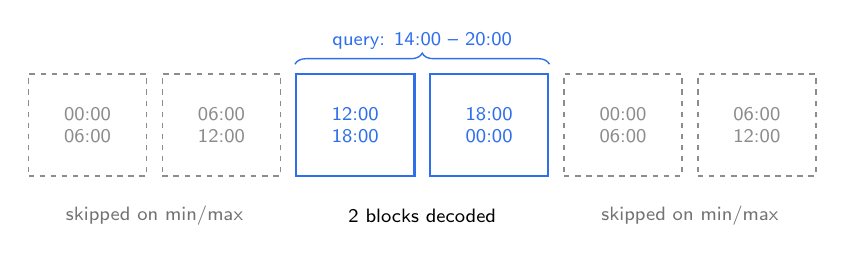
\begin{tikzpicture}[
  font=\small\sffamily, x=17mm,
  blk/.style={draw, line width=.6pt, minimum width=15mm, minimum height=13mm,
              inner sep=2pt, font=\scriptsize\sffamily, align=center},
  skip/.style={blk, dash pattern=on 2pt off 2pt, text opacity=.45, draw opacity=.45},
  scan/.style={blk, draw=accent, text=accent, line width=.9pt},
  lbl/.style={font=\scriptsize\sffamily, inner sep=2pt},
]
  \node[skip] (b0) at (0,0)  {00:00\\06:00};
  \node[skip] (b1) at (1,0)  {06:00\\12:00};
  \node[scan] (b2) at (2,0)  {12:00\\18:00};
  \node[scan] (b3) at (3,0)  {18:00\\00:00};
  \node[skip] (b4) at (4,0)  {00:00\\06:00};
  \node[skip] (b5) at (5,0)  {06:00\\12:00};

  \draw[decorate, decoration={brace, amplitude=4pt, raise=3pt}, line width=.5pt, draw=accent]
        (b2.north west) -- (b3.north east)
        node[lbl, midway, above=6pt, text=accent] {query: 14:00 – 20:00};

  \node[lbl, align=center] at (2.5,-1.15) {2 blocks decoded};
  \node[lbl, align=center, text opacity=.55] at (.5,-1.15)  {skipped on min/max};
  \node[lbl, align=center, text opacity=.55] at (4.5,-1.15) {skipped on min/max};
\end{tikzpicture}
